\chapter{Projektauftrag}

\label{AppendixProjektauftrag}

\section{Ausgangslage}\label{ausgangslage}

Als regelmässiger Konzertbesucher wünsche ich mir eine Plattform im
Internet, auf welcher ich eine zuverlässige Übersicht an Konzerten in
meiner Umgebung vorfinde. Heute sind die Events nur verteilt auf
verschiedenen Seiten wie die der Venues, des Konzertveranstalters, des
Künstlers oder auf Facebook publiziert.

Ich möchte deshalb eine zentrale Plattform entwickeln, die es Benutzern
einfach macht, Konzerte für ihren Geschmack zu finden.

Die Plattform soll Genre unabhängig sein und entsprechende Filter
anbieten.

Um einen zusätzlichen Service für den User zur Verfügungs zu stellen,
ist es auch denkbar, eine Art Notifikationssystem zu bauen um Benutzer
über Handy-Notifications oder per Email an Konzerte oder Künstler zu
erinnern.

Konzertveranstaltern kann das Erfassen ihrer Events vereinfacht werden,
indem auf der Plattform erfasste Veranstaltungen direkt auf den Sozialen
Medien wie Facebook, Twitter oder Instagram geteilt werden können.

\section{Projektziele}\label{projektziele}

\begin{longtable}[]{@{}lll@{}}
  \toprule
  Nr. & Zielbeschreibung\tabularnewline
  \midrule
  1.  & Webportal zum Auflisten und Suchen von Konzerten\tabularnewline
  2.  & Modernes responsives Design\tabularnewline
  3.  & Wird von Suchmaschinen indexiert\tabularnewline
  4.  & Inhalte des Portals sind durch die Benutzer erfassbar und bearbeitbar\tabularnewline
  5.  & Das Projekt muss bis Ende Mai 2019 abgeschlossen sein\tabularnewline
  \bottomrule
\end{longtable}

\subsection{Begründung der
  Projektziele}\label{begruxfcndung-der-projektziele}

\section{Terminplan}\label{terminplan}

Nachfolgend ist der grobe Terminplan für die geplanten Phasen. Im Anhang \ref{terminplan} ist
der detaillierte Terminplan abgelegt.

\begin{longtable}[]{@{}llr@{}}
  \toprule
  Phase           & Datum                   & Stunden\tabularnewline
  \midrule
  \endhead
  Initialisierung & 06.03.2019 - 31.03.2019 & 56\tabularnewline
  Konzept         & 01.04.2019 - 14.04.2019 & 58\tabularnewline
  Realisierung    & 22.04.2019 - 19.05.2019 & 112\tabularnewline
  Abschluss       & 20.05.2019 - 26.05.2019 & 36\tabularnewline
  \bottomrule
\end{longtable}

\clearpage

\section{Organigramm}\label{organigramm}

\begin{figure}[!htb]
  \centering
  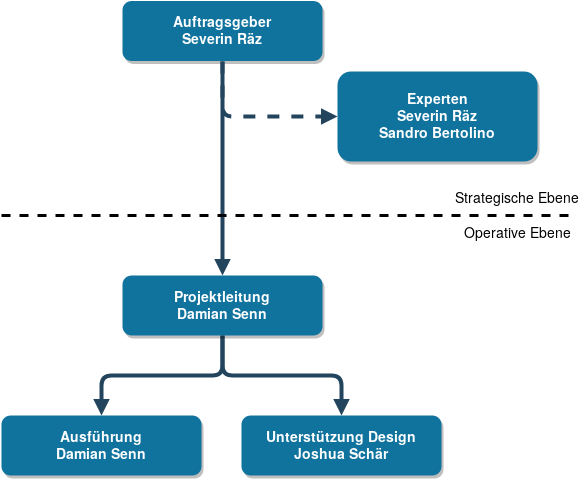
\includegraphics[width=0.8\textwidth]{figures/organigram.png}
  \caption{Organigram}
\end{figure}

\subsection{Tätigkeiten im Projekt}\label{tuxe4tigkeiten-im-projekt}

Für die Freigaben der Phasen ist nach Absprache mit Severin Räz Damian Senn
selbstständig verantwortlich.

\begin{longtable}[]{@{}ll@{}}
  \toprule
  Name             & Funktions- und Tätigkeitsbereich\tabularnewline
  \midrule
  \endhead
  Severin Räz      & Auftraggeber, externer Experte\tabularnewline
  Sandro Bertolino & Interner Experte\tabularnewline
  Damian Senn      & Projektleiter, Ausführung\tabularnewline
  \bottomrule
\end{longtable}

\clearpage

\section{Abgrenzungen}\label{abgrenzungen}

\begin{figure}[!htb]
  \centering
  \def\svgwidth{\columnwidth}
  \input{figures/abgrenzungen.pdf_tex}
  \caption{Abgrenzungen}
\end{figure}

\subsubsection{Hardware, Server-Installation, Deployment und
  Monitoring}\label{hardware-server-installation-deployment-und-monitoring}

Da das Projekt ein reines Software-Entwicklungs Projekt ist, werden
keine Operativen tätigkeiten wie Hardware beschaffung,
Server-Installation, Deployment und das einrichten eines
Monitoring-Systems vorgenommen.

\subsubsection{Datenschutz}\label{datenschutz}

Da das Projekt nicht deployed wird und somit nicht produktiv/online
gestellt wird, müssen im Rahmen dieser Projektarbeit noch keine Gedanken
über den Datenschutz gemacht werden.

\subsubsection{Datenimport}\label{datenimport}

Da wir bisher keine existierenden Konzertdaten besitzen, ist es nicht
nötig, einen Datenimport zu implementieren.

\subsubsection{Datenabfüllung}\label{datenabfuxfcllung}

Die Projektarbeit beinhaltet kein Datenset, Tests werden mit Testdaten
abgewickelt. Es liegt nicht in der Verantwortung des Projektleiters,
dass Daten in die Applikation abgefüllt werden.

\subsubsection{Backup Konzept}\label{backup-konzept}

Es wird kein Backup Konzept benötigt, da die Applikation im Rahmen
dieses Projektes nicht produktiv geschaltet wird.
